\chapter{实现与环境}

\section{实现平台与环境}
我们在\emph{gem5}模拟器上实现了MMT的原型,\emph{gem5}是一个多指令集的全系统模拟器,它可以模拟不同的指令集的(X86, ARM, RISCV, MIPS, SPARC等),不同的CPU模型:单周期,多周期,顺序执行,乱序执行,多发射等,不同的内存层次架构:
无缓存,L1缓存,L2缓存,L2缓存,以及指定每一级缓存的大小,集合,几路缓存等配置参数。同时gem5还对内存做了全模拟,实现了经典的内存模型以及ruby的内存模型。在模拟性能方面,gem5可以使用精确时间的模拟timing,原子的访问模拟atomic,以及性能的访问模式functional,
\emph{gem5}为全系统模拟提供了诸多搭配的选择,同时也提供了较为精确的模拟性能。相较于其他的相关工作使用的的trace模拟器(USIMM),只能够根据内存的访问trace文件,来进行模拟执行,这样的的模拟的精确性将不如全系统模拟。同时全系统模拟可能准确的执行程序并且
给出相应的计算结果,而不仅仅只是对性能的模拟。我们可以在\emph{gem5}上运行的完整的linux系统,或者未经过修改的原程序。
\begin{table}[htp]
    \centering
    \footnotesize
    \caption{\textbf{gem5中参数配置.}}
    \label{t:gem5-config}
    %\setlength{\belowcaptionskip}{0pt}
    %\begin{tabular}{@{}lll@{}}
    %\begin{tabular}{p{2.25cm}p{1.875cm}p{1.875cm}}
    \begin{tabular}{p{3.25cm}<{\centering} p{3.25cm}<{\centering} }
    %\begin{tabular}{@{}lrrrr@{}}
    \toprule
    \multicolumn{2}{c}{\textbf{处理器}} \\ \hline
    指令集              & RISCV    \\
    核数    &   4核 \\
    频率    &   1GZ \\
    L1d 缓存    &   两路,64K   \\
    L1i 缓存    &   两路,32K  \\
    L2 缓存    &   八路,2M  \\
    L3 缓存    &   十六路,16M  \\ \hline
    \multicolumn{2}{c}{\textbf{内存}} \\ \hline
    内存型号与频率    &   lddr3,800mHz \\
    读队列    &   32 \\
    写队列    &   64 \\
    行缓存    &   1K \\
    内存核心数    &   8 \\
    单通道rank数    &   2 \\
    单通道bank数    &   8\\ \hline
    \multicolumn{2}{c}{\textbf{内存时序参数}} \\ \hline
    Tck    &   1.25ns \\
    Tbust    &   5ns \\
    Trcd    &   13,75ns \\
    Tcl   &   13,75ns \\
    Tras    &   35ns \\
    Tcs   &   2.5ns \\
    \bottomrule
    \end{tabular} \\[-5pt]
\end{table}

如表格 ~\ref{t:gem5-config}所示,我们列举gem5配置的处理器,内存以及内存时序参数等。我们选择了指令集为RISCV的处理器,因为RISCV为开源指令集项目,可以方便做指令的修改以及后续的开发。同时市面上也存在诸多RISCV架构的处理和FPGA,能较为方便的从
模拟器中移植到真实的硬件中。我们采用了四核顺序处理的CPU核心,采用了三级缓存结构,其中L3缓存是共享的缓存。在内存控制器方面,内存控制器中的读队列和写队列分别为32和64。我们模拟了lddr3的内存,800mHz的频率,能够适应绝大多数的应用场景。其中单内存条(单通道)
上有两个rank,每个rank上拥有8个内存核心。其余的内存中刷新频率(Tck),行地址到列地址延迟(Tras)等相关信息可以具体参考表 ~\ref{t:gem5-config}

\begin{table}[htp]
    \centering
    \footnotesize
    \caption{\textbf{MMT中参数配置.}}
    \label{t:gem5-config}
    %\setlength{\belowcaptionskip}{0pt}
    %\begin{tabular}{@{}lll@{}}
    %\begin{tabular}{p{2.25cm}p{1.875cm}p{1.875cm}}
    \begin{tabular}{p{3.25cm}<{\centering} p{3.25cm}<{\centering} }
    %\begin{tabular}{@{}lrrrr@{}}
    \toprule
    \multicolumn{2}{c}{\textbf{MMT配置}} \\ \hline
    子树层数              & 三层   \\
    子树保护内存              & 4M   \\
    根数层数              & 三层   \\
    子树保护内存              & 2M   \\
    MMT元数据区域              & $\approx$2M   \\
    SoC保护内存大小              & 128M   \\
    最大保护内存大小              &  512G   \\
    Mount Table              & 16K   \\
    Secure Bitmap   & 512B \\
    \bottomrule
    \end{tabular} \\[-5pt]
\end{table}

\section{gem5模拟器}
我们在了gem5中的$dram_ctrl$,实现了MMT的原型,为了能够更精确的模拟内存访问的时间,我们选择了Timing模式,Timing模式能够实现原子的内存访问请求,从而更加的精确的计算CPU到内存的延时。gem5是事件驱动的模拟,通过调度器合理的触发事件队列中待完成的事件。
事件包括:Cache想内存控制器发送一个内存访问的数据包,内存进行预充电,将写入内存的数据加入到内存控制器中的写缓存中等等。同时,gem5中不同硬件部件之间的通信时通过包的机制进行的,每一个能够接受消息的部件都会预留四个接口,在Timing模式下为:$recvTimingReq()$,$sendTimingReq()$,$recvTimingResp()$,$sendTimingResp()$,例如cpu中向cache中读取数据,cpu会生成一个包含cache地址,访问权限以及预留
数据的空间等其他包元数据,然后将这个数据包发送给cache单元。在cache单元中$recvTimingReq()$和cpu中的$sendTimingReq$通过管道的机制连接在一起,所以从cpu中的消息可以传到cache中。值得注意的时,cpu中发送消息包会触发一个事件,该事件会加入掉调度的队列中,并且在它该触发的时候执行。例如cpu访问cache需要几个cycles的时间,那么cpu中发送的数据包给cache这个事件就会在对应的cycle数之后才会被调度到。同样道理如果发生
cache miss 数据要从内存中获取时候,cache会生成了一个内存访问的数据包,该数据的包获取数据的大小和一个内存块或缓存行的大小相同,然后将cache向内存控制器发送请求包的事件加入调度队列中,该事件会在一定的延时后触发(模拟cache到内存控制器的延时),当内存控制器获取
数据之后,会填充在请求包的数据区间,然后将包返回给cache,该过程也会产生一个事件,并且在特定的时间点触发。cache即获得了内存中的数据,然后更新cache缓存行中的数据,然后将结果返回给cpu。这就是在gem5中运用包机制以及事件驱动完成对全系统的模拟。

另外gem5对硬件的模拟非常的精准与细致。在cpu上可以模拟不同指令集的cpu核心,在同一个指令集中,也有多种模式可以选择:单周期,多周期,乱序,Timing,atomic等等。在cache方面,可以模拟L1,L2,L3缓存,同时缓存中的集合数以及路数都可以配置,在L1缓存中还区分数据块和代码块,L3cache实现了cache一致性的协议。在内存部分,可以实现丰富的内存模拟,
包括内存的频率(1600、2400);不同的内存种类(lddr4、lddr4、hmc),不同的内存核心数量,rank和bank的数量,输出引脚的数量等等。除了能够模拟多种内存的模型,还能够精确设置内存性能至关重要的时序参数,例如:Tck、Tras等等。表格 ~\ref{t:gem5-config}中列举了我们模拟中采用的硬件,同时在测试的时候,我们也尝试使用不同的硬件组合,来测试程序运行是的性能。

\section{内存控制器}
内存控制处在SoC上,连接着总线。一个内存控制器控制着一个DIMM,能够触发对内存条的读写指令;当同时存在多个DIMM并插有多个内存条时,就需要有SoC中有多个与之对应的内存控制器。为了使内存控制器能够实现MMT的功能,我们在原始的gem5内存控制器上进行了进一步的修改,增加了内存控制器中的三个组件:Secure Bitmap;Mount Table;Root-of-root,另外我们还针对子树和根数节点设计了缓存结构(Tree Node Cache),能够进一步换件完整性检查时候访问内存的开销。
最对Secure Bitmap,我们在内存控制初始化的时候分配了16K的内存,其中每一个bit代表一颗子树是否被分配,初始化的时候我们将Secure Bitmap全部清零。在初始化阶段,我们还要分配Mount Table和Tree Node Cache的内存。其中Mount Table为四个集合,每一个集合中有两路缓存行,一个Mount Table 缓存行中可以存放4个子树的节点,Mount Table的大小为512B能够存储32颗子树。每一个Mount Tablew的缓存行组织结构如下~\ref{fig:Mount-Table-Set.png}所示:

\begin{figure}[!htp]
    \centering
    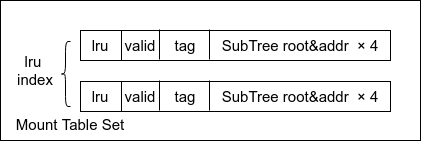
\includegraphics[scale=0.5]{Mount-Table-Set.png}
    \caption{\textbf{Mount-Table-Set }Mount Table缓存行中的数据结构}
   \label{fig:Mount-Table-Set.png}
\end{figure}
Mount Table Set中一个缓存行由四个部分组成,分别是lru bit,valid bit,tag,以及子树的根节点信息。其中lru bit记录了当前的缓存行最近是否被访问过,如果被访问锅则lru bit被设置为1,如果没有被访问过,则lru bit被设置为0.如果lru bit为0表示当前的缓存行能够被驱逐出去。valid bit表示当前的缓存是否有效,如果为1表示当前的缓存中的数据是有效的,可以被内存控制器之间读取。tag是用于区分相同缓存集合中不同的缓存行,只有tag匹配一直且valid bit为1才被人为是缓存命中。
一个缓存行中存储了四个子树的节点,其中每个子树根节点的大小为16B,包括了子树的counter以及地址。

在gem5的内存控制器中,通过$recvTimingReq(PacketPtr pkt)$接受来自cache的数据包,通过$port.schedTimingResp(pkt, response_time)$将读取的数据返还给cache。当内存控制器接受到数据包的时候,首先会检查对应内存是否需要完整性保护$checkSecureBItmap$,如果访问的内存不需要完整性保护则调用$recvTimingReqNonSecure(pkt)$,如果需要完整性保护则回去Mount Table中寻找对应的子树根节点,如果子树的根节点不在Mount Table中那么,会去MMT元素局区域获取
子树的根节点$acquireSubTreeNode(pkt)$,并且将从Mount Table中淘汰的子树的节点更新到MMT元数据区域中,同时更新Root-of-root的数值。当子树的根节点在Mount Table中,内存控制器能够进行之后的完整性检查。首先内存控制器会检查该数据包包含的内存访问是读请求还是写请求:$pkt->isWrite()$,$pkt->isWrite()$,如果是读请求,则将数据包放入内存控制器中的读缓存队列中,如果是写请求,则将数据包放入写缓存队列中。当数据包在读缓存队列中的时候,回去检查之前的
写缓存队列中是否存在相同内存地址的写请求,如果存在,那么可以直接将写请求中的数据放入读请求的数据包中,返回给cache。如果读请求的数据包对应的内存地址不在写缓存队列中,那么将会发起一次内存的读操作。为了保证内存中数据的完整性,我们还需要读取对应内存的子树中的节点。我们首先会去保存子树的节点的缓存中检查对应的子树节点是否在Tree Node Cache中,如果在Tree Node Cache中那么可以直接读取到对应的子树节点中的counter和hash(会根据子树的层数以及内存的地址计算对应的counter在子树节点中的offset),
如果不在Treee Node Cache中,则需要额外做一次内存的访存请求。所有的内存读写请求都会生成一次事件,加入到事件的调度其中。当读写内存请求的事件被调度到时,内存控制器会调用$processRespondEvent()$处理从内存中读到的数据。首先内存控制器会区分读取的数据是子树节点中的数据还是原本内存请求中的数据。当所有的子树节点中都在内存控制器中可读到时候(要么在Tree Node Cache中,要么从内存中读取出来),内存控制器会进行根据子树的节点对内存中的数据做完整性检查。
如果完整性检查成果,则内存中的数据写到数据包中,调用$port.schedTimingResp(pkt, response_time)$,将结果返回给cache。对于数据包中的请求是写请求的话,将数据包加入写缓存队列,并将写内存事件加入事件调度器中,内存控制器会去更新对应子树中counter值,然后通知cache,内存写请求更新完成。因为一旦数据包静茹了写队列,之后的读求情都会先在写队列中寻找是否存在对应的数据,写队列的中的数据包也会异步的刷到内存中。
